\chapter{Analyse}

\section{Analyse de la relaxation}
\graphicspath{{04-Analyse/}}
\minitoc
Le processus de relaxation utilisé dans l'algorithme CxSOM est une méthode originale pour construire des connexions bidirectionnelles entre cartes. Deux cartes connectées de cette façon jouent alors un rôle symétrique, contrairement à une connexion unidirectionnelle ou hiérafchique ou une carte joue le rôle d'entrée. Dans cette section, nous évaluons expérimentalement la méthode de relaxation en tant que moyen de trouver une Best Matching Unit cohérente. On cherchera notamment à répondre aux questions suivantes :  
\begin{itemize}
\item Est-ce que la méthode de relaxation converge ?
\item Est-ce que que cette méthode est déterministe ?
\item Quels sont les paramètres à prendre en compte dans l'algorithme de relaxation ?
\end{itemize}

\subsection{Formalisation de la relaxation}

La relaxation est une recherche de point fixe de l'activité globale de chaque carte de l'architecture. Notons $(\mathbf{\bmu})_\tau = (\bmu\m{0}_\tau,\cdots,\bmu\m{N}_\tau)$ la suite définie par l'évolution des BMUs des $N$ cartes d'une architecture lors de la relaxation.
La suite $(\mathbf{\bmu})_\tau$ est une suite définie par récurrence par $\mathbf{\bmu}_{\tau+1} = \mathbf{f}(\mathbf{\bmu}_\tau)$
avec $\mathbf{f} = (f\m{0},\cdots,f\m{N}) : [0,1]^N \rightarrow [0,1]^N$ une application non linéaire transformant l'espace des positions des BMUs; $\mathbf{f}$ ne dépend pas de $\tau$.


Détaillons l'évolution de cette suite. Pour clarifier les notations, définissons pour chaque carte~$i$:
\begin{equation}
\begin{gathered}
p\star\m{i}_{\tau} = \argmax_{p\m{i}}(a_g\m{i}(p\m{i},\bmu\m{i_0}_\tau, \cdots \bmu\m{i_K}_\tau))\\
 i_0, \cdots i_K \: \text{indices des cartes nourrissant la carte $i$}.
\end{gathered}
\label{eq:pstar}
\end{equation}
$a_g\m{i}$ est une fonction des poids de la carte $\w\ext\m{i}, \w\cont\m{i}$ et de son entrée externe $\inpx\m{i}$. Lors du processus de relaxation, les poids et l'entrée restent fixes. Le calcul de $a_g$ ne dépend pas de $\tau$.
Pour toute carte $i$, $p\star\m{i}_{\tau}$ est donc seulement une fonction de $(\bmu\m{i_0}_\tau, \cdots \bmu\m{i_K}_\tau)$.
L'équation d'évolution s'écrit alors: 
\begin{equation}
\bmu\m{i}_{\tau+1} = 
\begin{cases}
\bmu\m{i}_{\tau} + sgn(p\star\m{i}_{\tau} - \bmu\m{i}_{\tau}) \times \delta \; & \text{si $p\star\m{i}_{\tau} - \bmu\m{i}_{\tau} > \delta$ } \\
p\star\m{i}_{\tau} \; \text{sinon}	
\end{cases}
\label{eq:evolution}
\end{equation}

En posant $f\m{i}$ la partie droite de l'équation \ref{eq:evolution}, on peut donc écrire: 
\begin{equation}
\bmu\m{i}_{\tau +1} = f\m{i}(\bmu\m{0}_\tau,\cdots,\bmu\m{N}_\tau)
\label{eq:fonction}
\end{equation}
Soit, pour l'ensemble des composantes : 
\begin{equation*}
\mathbf{\bmu}_{\tau+1} = \mathbf{f}(\mathbf{\bmu}_\tau)
\end{equation*}
L'état initial $(\bmu\m{0}_0, \cdots , \bmu\m{N}_0)$ est défini dans CxSOM par: 
\begin{equation}
\begin{cases}
\bmu\m{0}_0 = \argmax_{p\m{0}} a_e(p\m{0},\inpx\m{0})\\
\cdots \\
\bmu\m{N}_0 = \argmax_{p\m{N}} a_e(p\m{N},\inpx\m{N})\\
\end{cases}
\label{eq:init}
\end{equation}

La relaxation se traduit ainsi par une recherche de point fixe de la suite $(\mathbf{\bmu})_{\tau}$, soit une position $\mathbf{\bmu}$ telle que:
\begin{equation}
\mathbf{\bmu} = \mathbf{f}(\mathbf{\bmu})
\label{eq:suite}
\end{equation}

Si $f$ admet un point fixe, alors ce point fixe est aussi un point fixe pour la suite $(\mathbf{\bmu})_\tau$. Cependant, rien ne garantit que ce point fixe existe, et qu'il sera atteint par la suite.
Expérimentalement, il semble que si $\mathbf{f}$ admet un unique point fixe, alors $(\mathbf{\bmu})_{\tau}$ converge vers ce point fixe. On montrera que ce point fixe n'est pas toujours unique, notamment lorsque les poids sont aléatoires au début de l'apprentissage, ce qui entraîne alors une non-convergence de la relaxation. Cependant, ces cas de non-convergence n'influencent pas l'apprentissage des cartes en choissant des bons paramètres d'apprentissage. On observera expérimentalement qu'à la fin de l'apprentissage, la disposition des poids permet l'existence d'un unique point fixe. 


\subsection{Etude de la convergence des BMUs lors de la relaxation}

La méthode de relaxation cherche la convergence des BMUs de l'architectures. Nous avons donc réalisé 1000 itérations de test, à poids figés, à différents temps d'apprentissage, et comptons le nombre de pas nécessaires à la convergence de la relaxation. L'algorithme utilisé pour la relaxation s'arrête automatiquement si la relaxation dépasse $\tau_{max}= 1000$ itérations. On considérera que la relaxation n'a pas atteint un point de convergence si la relaxation atteint ces $\tau_{max}$ itérations.
Théoriquement, plusieurs situations se traduisent par une non-convergence de la relaxation:
\begin{itemize}
\item La relaxation évolue vers un point de convergence, mais trop lentement pour y arriver en moins de 1000 itérations
\item La relaxation évolue vers un cycle limite composé d'un nombre limité d'unités étant alternativement best matching units
\item La relaxation évolue sans répétition de motifs dans la carte : évolution chaotique.
\end{itemize}
Le premier cas est évité car la limite de 1000 itérations est assez grande par rapport à la taille de la carte, les cartes sont de tailles 500. Le pas d'évolution de la relaxation est d'une dizaine d'unités. La convergence, si elle existe, est donc rapide. Nous observerons plus précisément les trajectoires dans la section suivante; on s'intéresse ici seulement à la question de la convergence.
L'étude de la convergence sera réalisée dans des architectures de 2 et 3 cartes, pour des cartes une dimension et deux dimensions.

La figure \ref{fig:conv_evolution} présente l'évolution du taux de convergence au cours de l'apprentissage d'une architecture de 2 cartes et 3 cartes. La figure \ref{fig:conv_evolution2D} trace  cette évolution dans le cas ou les cartes sont en 2 dimensions. Pour tracer cette évolution, on effectue des étapes de tests à intervalles réguliers au cours de l'apprentissage, pendant lesquels les poids ne sont pas mis à jours. Ces tests sont réalisés sur 1000 entrées externes $X,Y$ (et $Z$ pour trois cartes), prises aléatoirement dans l'espace d'entrée. On prélève, pour chaque échantillon de test, le nombre de pas nécessaire à la relaxation. Si ce nombre est égal à $\tau_{max}$, on considère que la relaxation n'a pas convergé. On trace alors, en haut, le pourcentage d'échantillons de test pour lesquel la relaxation converge. En bas, on trace le nombre moyen de pas de relaxation nécessaires à la convergence.
Dans chaque cas, on répètera 10 fois l'apprentissage, et on trace la moyenne et écart type des valeurs obtenues sur ces 10 répétition.

Au début de l'apprentissage, lorsque les poids sont aléatoirement initialisés, la relaxation atteint rarement un point de convergence. Lorsque les cartes se déplient, la relaxation évolue vers un point de convergence dans plus de $90 \%$ des cas. Cette évolution est similaire pour des architecture de deux et trois cartes. Les expériences avec des cartes en deux dimensions présentent la même évolution. Le taux de convergence en fin d'apprentissage est plutot situé entre $80 \%$ et $90 \%$.
 
\begin{figure}
\centering
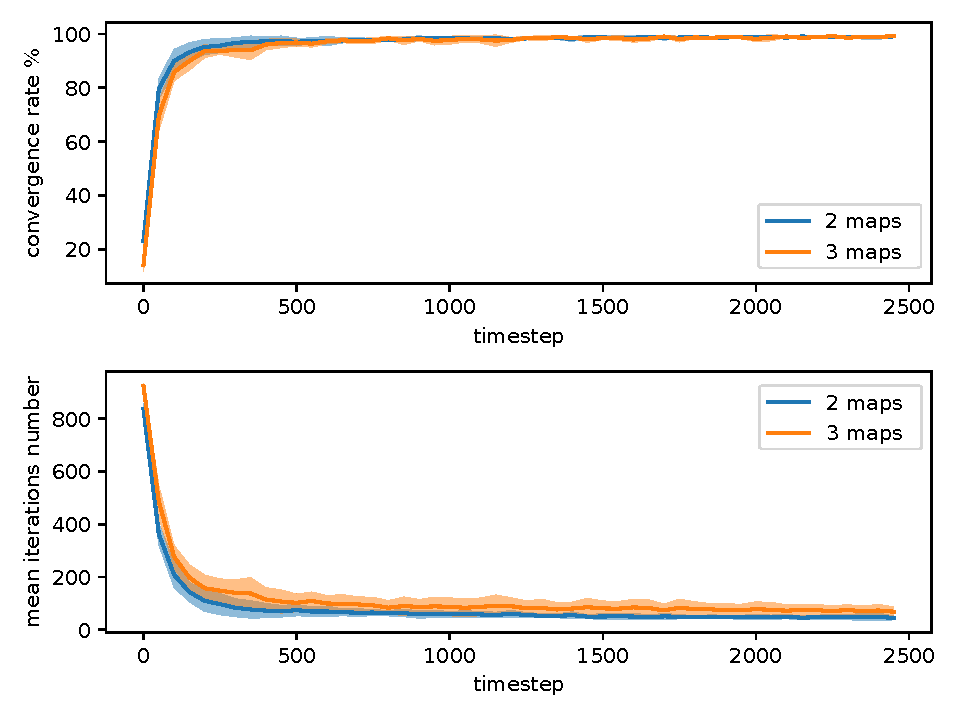
\includegraphics[width=0.7\textwidth]{1D_conv_evolution_total.pdf}
\caption{Evolution du taux de convergence moyen lors de la relaxation au cours de l'apprentissage sur deux et trois cartes 1D. Chaque point est calculé sur un échantillon de 1000 relaxations au temps t, évaluées sur des entrées différentes prises aléatoirement sur le cercle. Moyenne et écart-types calculés sur 10 expériences.}
\label{fig:conv_evolution}
\end{figure}


\begin{figure}
\centering
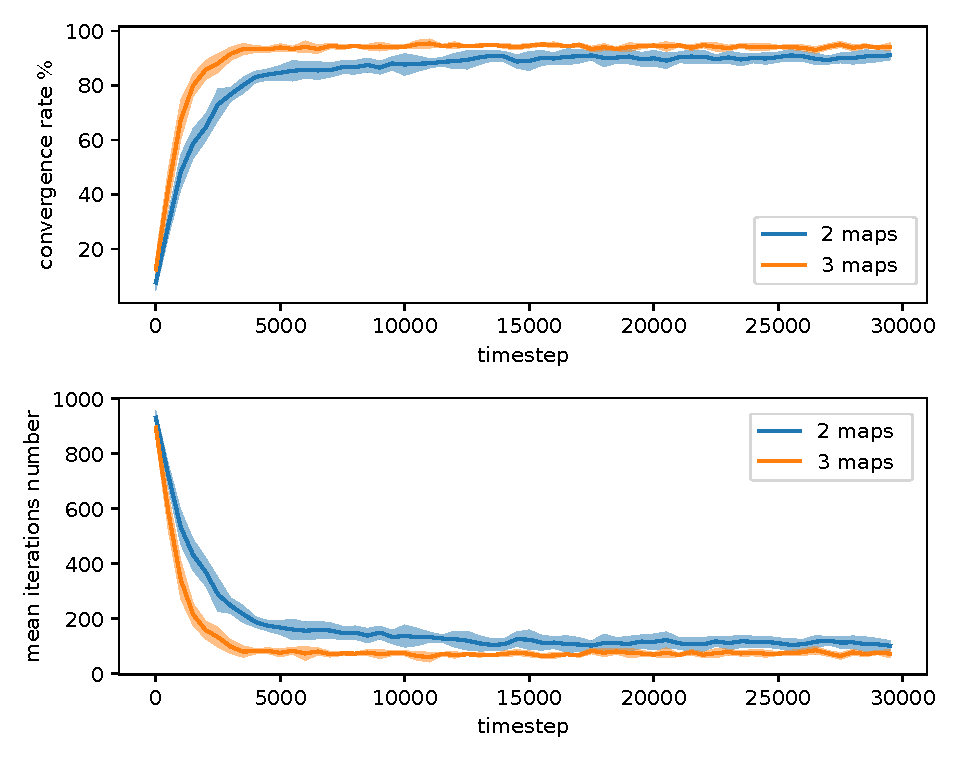
\includegraphics[width=0.7\textwidth]{2D_conv_evolution_total.pdf}
\caption{Evolution du taux de convergence moyen lors de la relaxation au cours de l'apprentissage sur deux et trois cartes 2D. Chaque point est calculé sur un échantillon de 1000 relaxations au temps t, évaluées sur des entrées différentes prises aléatoirement sur le cercle. Moyenne et écart-types calculés sur 10 expériences.}
\label{fig:conv_evolution2D}
\end{figure}

\subsection{Etude de l'influence de l'entrée contextuelle sur le BMU}

Dans cette section, nous étudions plus précisément l'évolution de la suite $(\mathbf{\bmu})_{\tau}$ dans le cas de d'une architecture de deux cartes connectées. Les cartes sont $M\m{1}$ et $M\m{2}$ prenant en entrée externe respectivement $\inpx\m{1} = X, \inpx\m{2} = Y$.
Les entrées contextuelles des deux cartes sont à valeurs dans l'espace des positions d'une carte: $\inpc\m{1} = \bmu\m{2}$ et $\inpc\m{2} = \bmu\m{1}$
On définit donc les valeurs $p\star\m{1}$ et $p\star\m{2}$ comme indiqué dans l'équation \ref{eq:pstar}
\begin{equation} 
\begin{cases}
	p\star\m{1}_{\tau} = \argmax_{p\m{1}}(a_g(p\m{1},\bmu\m{2}_{\tau}) \\
	p\star\m{2}_{\tau} = \argmax_{p\m{2}}(a_g(p\m{2},\bmu\m{1}_{\tau}) \\
\end{cases}
\end{equation}

On tracera les valeurs de $p\star\m{1}$ en fonction de son entrée contextuelle $\bmu\m{2} \in [0,1]$, et $p\star\m{2}$ en fonction de $\bmu\m{1} \in [0,1]$ en figure \ref{fig:w006}.
Cette expérience est réalisée après l'apprentissage. On remarque que, $p\star\m{i}$ varie peu en fonction de l'entrée contextuelle de la carte; la relaxation se déroulera donc dans une partie réduite de la carte.

On peut comparer ces tracés à ceux réalisés au début de l'apprentissage ($t=0$), lorsque les poids sont aléatoires, et pendant l'apprentissage ($t=150$). Pour $t=150$, les poids externes ont déjà convergé, mais pas encore les poids contextuels, car le rayon de voisinage utilisé pour les poids contextuel est bien plus faible que pour les poids externes.
%TODO tracés (cercle 006)

\begin{figure}
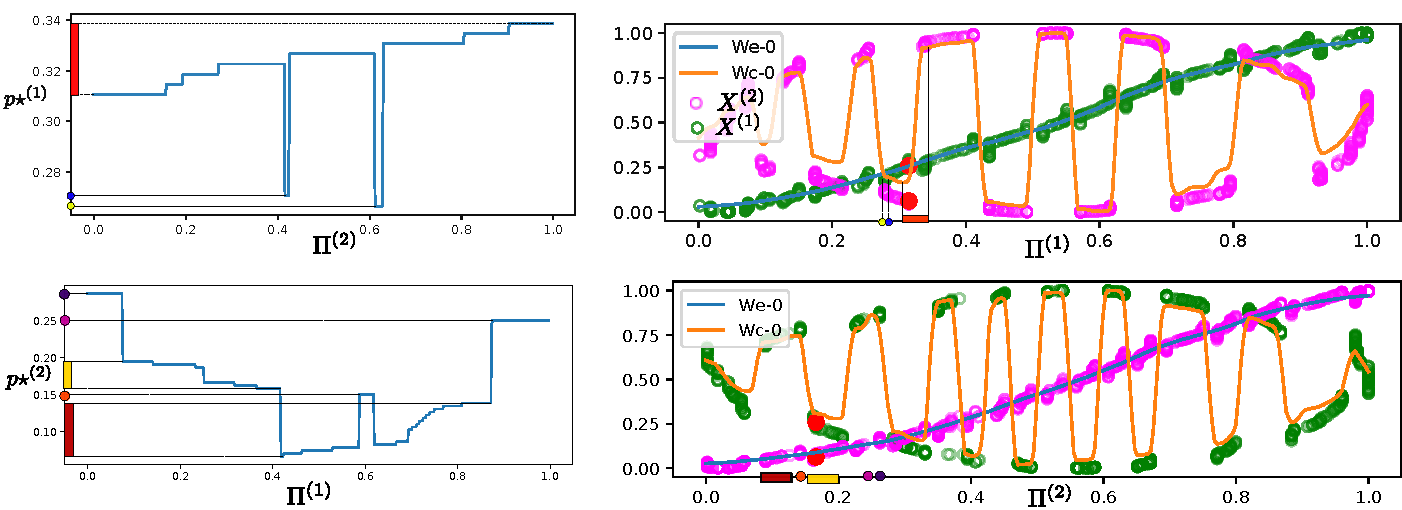
\includegraphics[width=\textwidth]{am_w_006}
\caption{A gauche, $p\star\m{1}$ et $p\star\m{2}$ en fonction de l'entrée contextuelle de leur carte $\bmu\m{2}$ et $\bmu\m{1}$. A droite, les poids externes et contextuels des cartes $1$ et $2$ sont représentés selon leur position dans la carte. On représente également les entrées test $\inpx\m{1}$ et $\inpx\m{2}$ en fonction de leur BMU. Les entrées utilisées pour tracer les figures de gauche sont colorées en rouge sur les figure de droite: $\inpx\m{1}=0.26,\inpx\m{2}=0.06$}
\label{fig:w006}
\end{figure}


\subsection{Etude de l'unicité du point fixe}

Considérons 
On étudiera donc l'évolution de processus de relaxation lancés sur les mêmes poids, pour une entrée externe fixée, intialisés à des valeurs aléatoires de BMU dans chaque carte.
Chacun de ces processus aboutit sur un point de convergence; on tracera donc la distance moyenne entre les différents points de convergence sur toutes les expériences. Si cette distance est nulle, alors le point de convergence est un point fixe qui ne dépend pas de l'initialisation. 
Cette étude sera réalisée sur des cartes 1D et 2D, pour des architectures de 2 et trois cartes.

\begin{figure}
\begin{minipage}{0.5\textwidth}
\centering
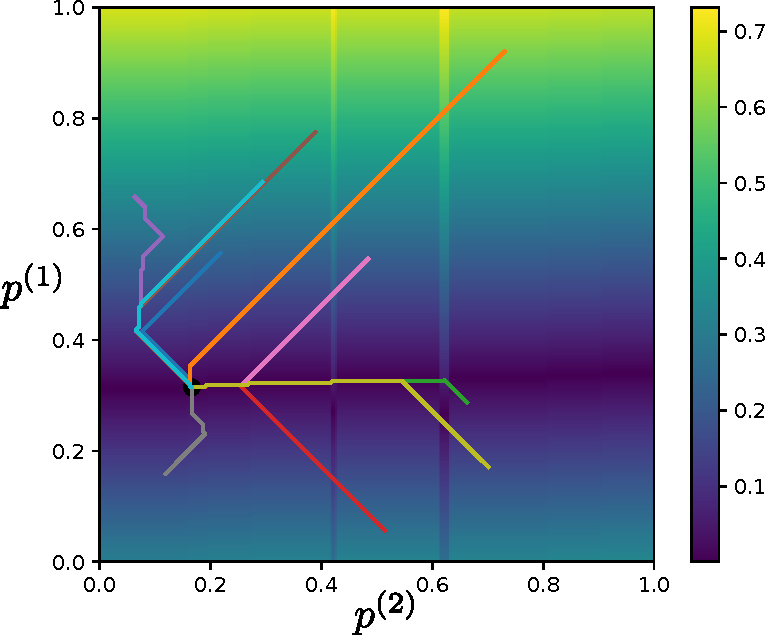
\includegraphics[width=\textwidth]{champ_X_006.pdf}
\end{minipage}
\begin{minipage}{0.5\textwidth}
\centering
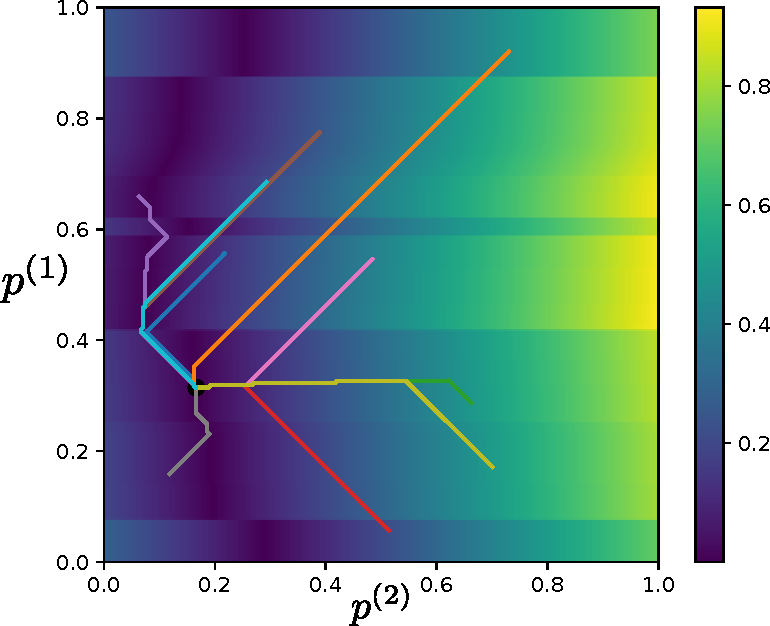
\includegraphics[width=\textwidth]{champ_Y_006.pdf}
\end{minipage}
\caption{Valeur de ${p\star}\m{1} - p\m{1}$, resp. ${p\star}\m{2} - p\m{2}$. ${p\star}\m{1}$ ne dépend que de $p\m{2}$ : on peut donc tracer cette valeur selon deux dimensions pour chaque carte. Les zones où cette valeur est nulle sont en violet sur le graphique. Les points fixes, s'il existent, sont aux positions de différence nulle pour $M\m{1}$ et $M\m{2}$.}
\label{fig:diff_relax}
\end{figure}

\begin{figure}
\begin{minipage}{0.5\textwidth}
\centering
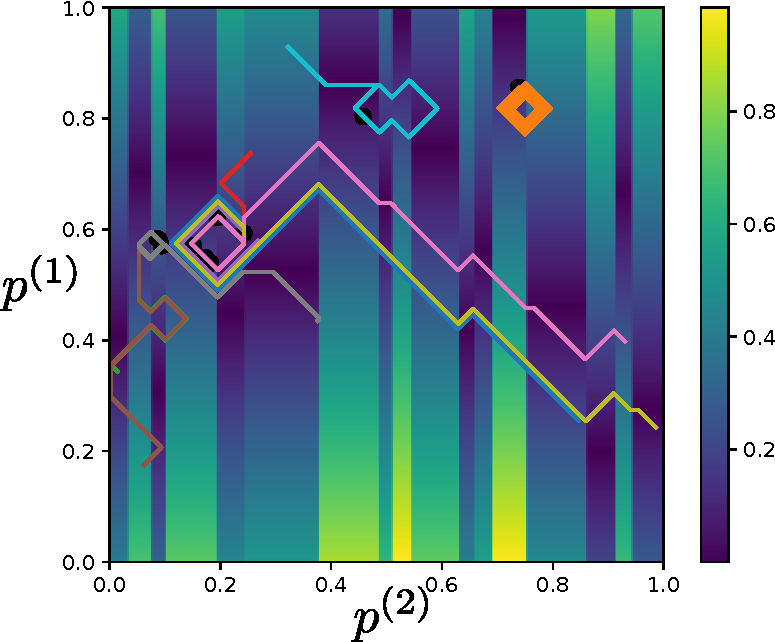
\includegraphics[width=\textwidth]{champ_X_006_t1.pdf}
\end{minipage}
\begin{minipage}{0.5\textwidth}
\centering
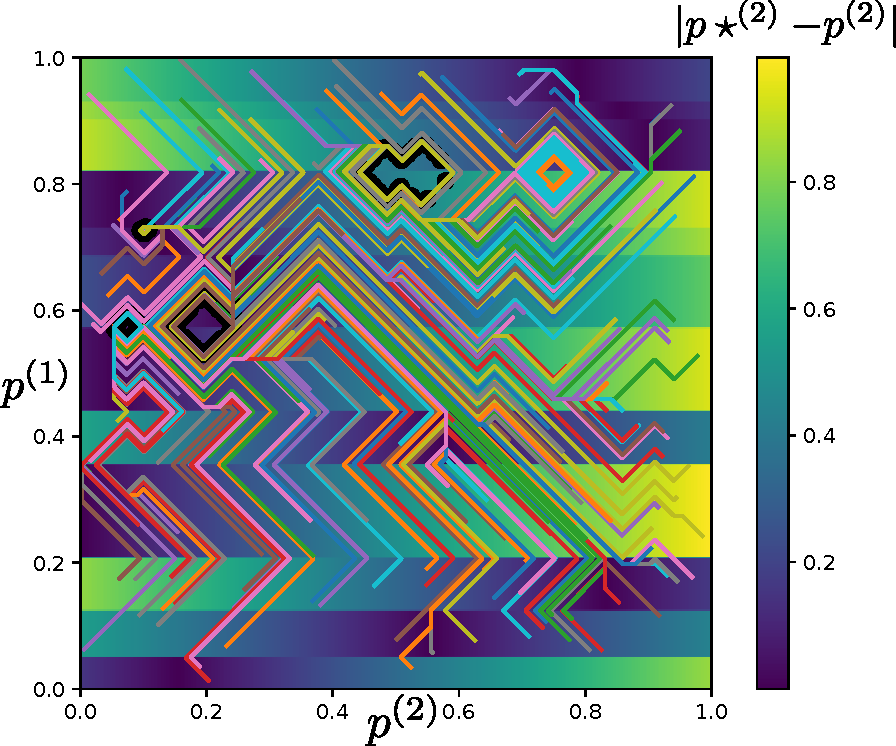
\includegraphics[width=\textwidth]{champ_Y_006_t1.pdf}
\end{minipage}
\caption{Valeur de ${p\star}\m{1} - p\m{1}$, resp. ${p\star}\m{2} - p\m{2}$. ${p\star}\m{1}$ ne dépend que de $p\m{2}$ : on peut donc tracer cette valeur selon deux dimensions pour chaque carte. Les zones où cette valeur est nulle sont en violet sur le graphique. Les points fixes, s'il existent, sont aux positions de différence nulle pour $M\m{1}$ et $M\m{2}$.}
\label{fig:diff_relax_t1}
\end{figure}

\begin{figure}
\centering
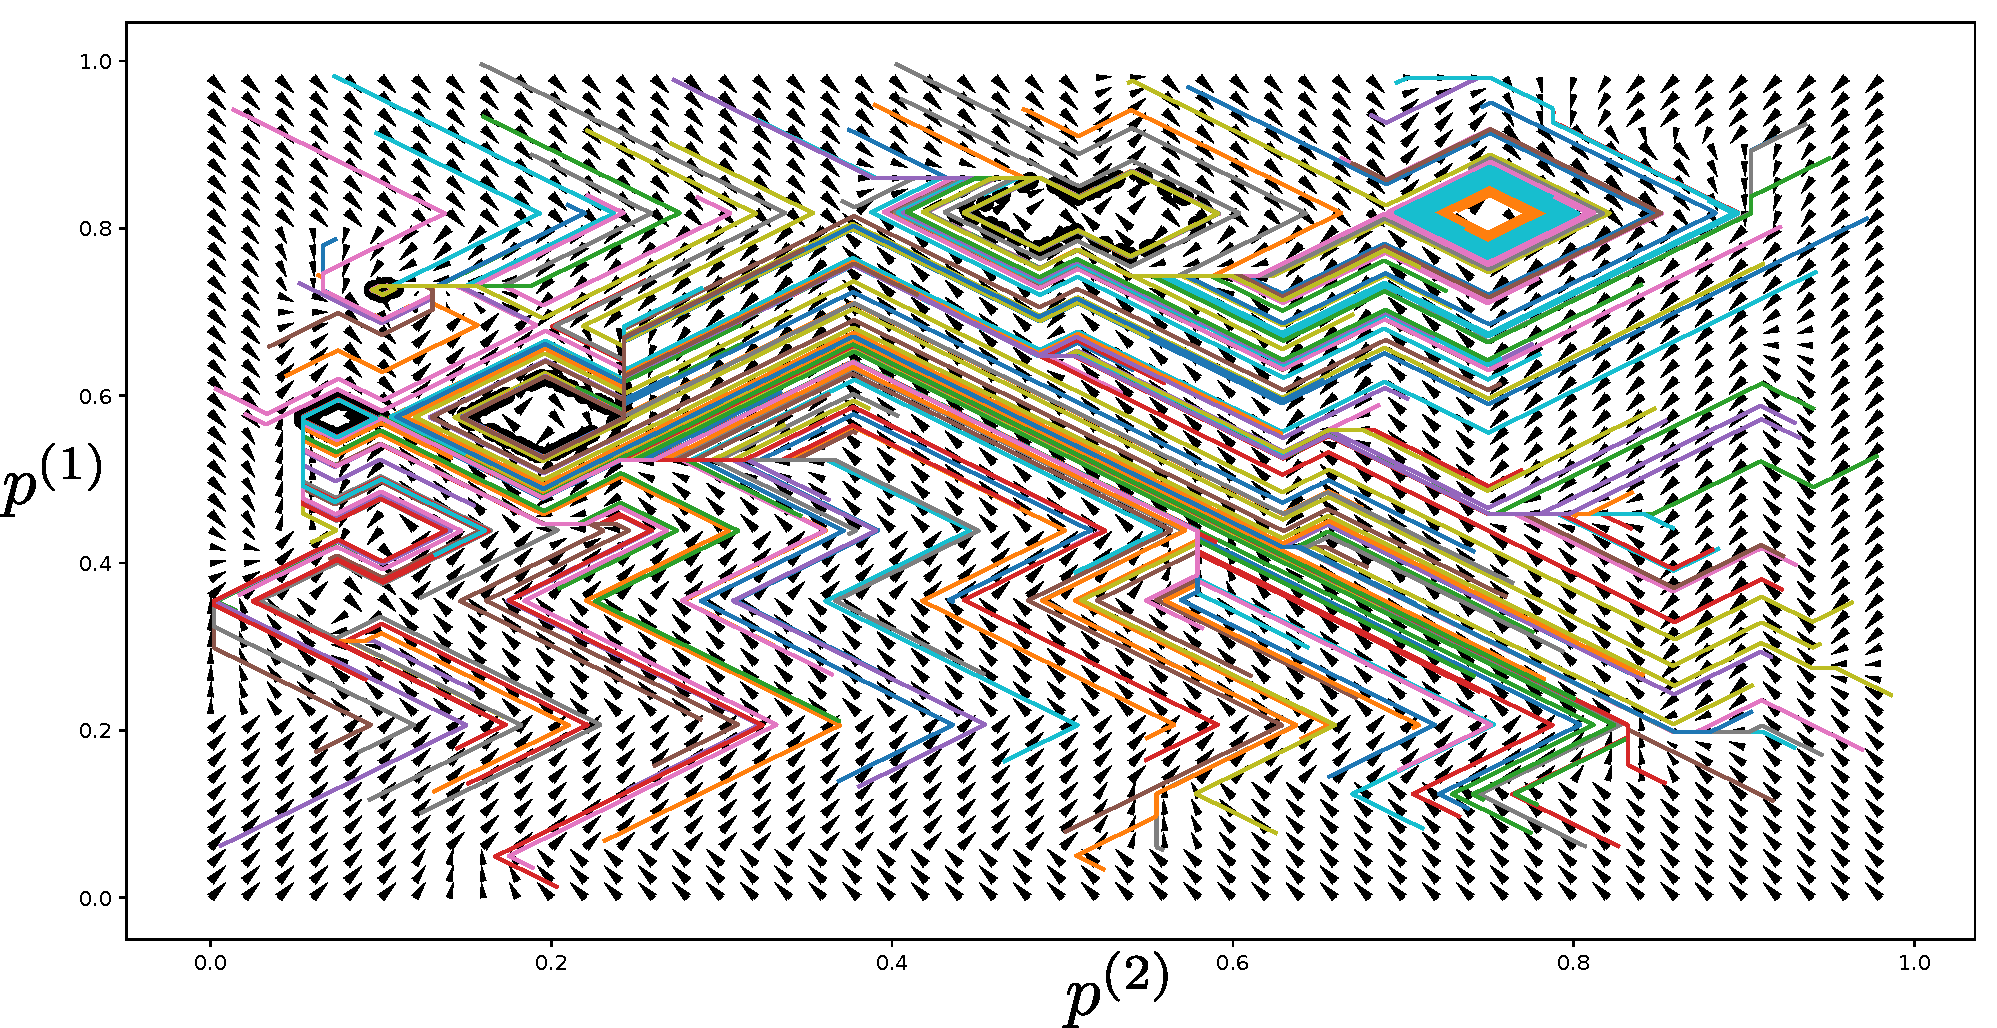
\includegraphics[width=\textwidth]{champ_006_t1.pdf}
\end{figure}


\begin{figure}
\centering
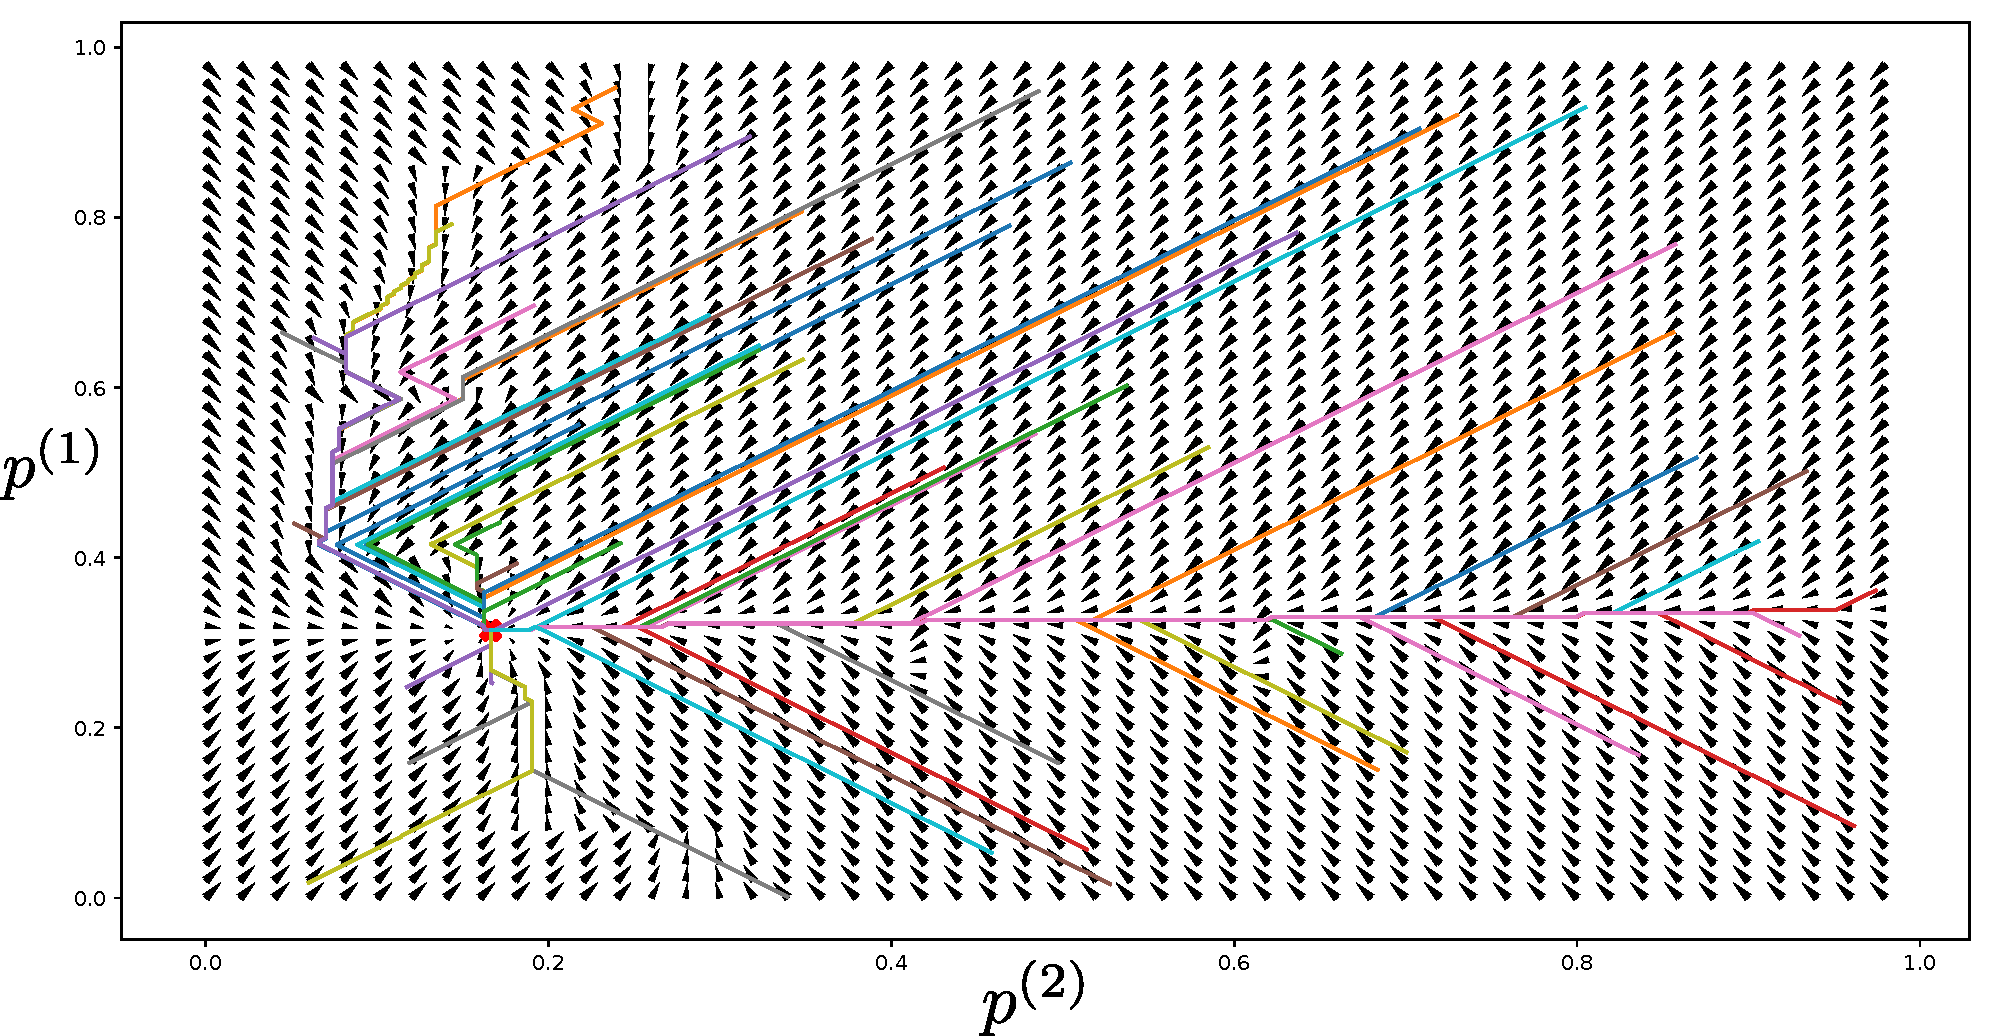
\includegraphics[width=\textwidth]{champ_006.pdf}
\end{figure}

\subsection{Discussion}

\draft{
\begin{itemize}
\item Element clé de l'architecture : relaxation. A t-on toujours un point de convergence ? Sinon, dans quels cas ? 
\item On peut tracer les champs de relaxation pour trouver le point fixe. 
\item Une carte est un système dynamique comme une variable passant d'un état à un autre. Etat = BMU.
\end{itemize}
}


\section{Analyse de l'auto-organisation}